\documentclass[authordate, anecdote]{jote-new-article}

\usepackage{caption}

\usepackage{tabularx}

\usepackage{graphicx}

\usepackage{hyperref}

\usepackage[backend=biber,style=apa]{biblatex}

\addbibresource{bibliography.bib}

\jotetitle{The Popcorn Effect: A Serendipitous Discovery in Thermal Biomass Gasification}
\keywordsabstract{biomass, renewable energy, chemical engineering, models in engineering, philosophy of science}
\runningauthor{Roßmann}
\jname{Journal of Trial \& Error}
\jyear{2025}
\paperdoi{10.36850/e1c8-4c62}
\paperreceived{September 16, 2024}
\author[1]{\mbox{Maximilian Roßmann\orcid{0000-0002-0499-030X}}}
\affil[1]{Maastricht University, Maastricht, the Netherlands}
\corremail{\href{mailto:m.rossmann@maastrichtuniversity.nl}{m.rossmann@maastrichtuniversity.nl}}
\corraddress{Maastricht University}
\runningauthor{Roßmann}
\paperaccepted{November 10, 2024}
\paperpublished{March 3, 2025}
\paperpublisheddate{2025-03-03}
\jwebsite{https://journal.trialanderror.org}

\begin{document}
\begin{frontmatter}
  \maketitle
  \begin{abstract}
    \printabstracttext
  \end{abstract}
\end{frontmatter}


	\section{Introduction: The energy transition and a bachelor's thesis}



	This is the story of my serendipitous invention of a popcorn effect in thermal biomass gasification and the role of scientific imagination. In 2011, during my time at the Fraunhofer Institute for Solar Energy Systems (ISE) in Freiburg, I embarked on a project that would unexpectedly lead to a small discovery. Nestled in a city known for its open-minded student culture and scenic Black Forest hikes, I found myself immersed in the world of thermic biomass gasification—a process, back then, considered promising for the energy transition. My journey began with a bachelor's thesis aimed at understanding the reduction reactions in pyrolyzing wood pellets with minimal oxygen at high temperatures, ultimately fueling combined heat and power (CHP) units to contribute to the energy transition. Surrounded by young engineers studying cutting-edge technologies like Redox flow batteries and photovoltaic cells, I felt a part of a larger mission.



	The main promises of thermal biogas gasification are its flexible energy production and feedstock. Burnable gases can be stored efficiently and utilized flexibly during periods when the winds don't blow and the sun does not shine. Unlike traditional biogas plants, thermal gasification can process a wider variety of biomass that is less amenable to fermentation, such as municipal waste or sewage sludge. Integrating such a process into sewage treatment, which was the aim of the follow-up project, could reduce transport costs and allow the recovery of phosphorus, a finite resource, promoting a circular economy (Lintner et al., 2012; Tan \& Lagerkvist, 2011). However, because the prices of photovoltaic (PV) and wind turbines decreased drastically (Roser, 2020) and economic incentives to recycle phosphorus remained insignificant, thermal biomass gasification is still an emergent niche technology.



	\section{The experiment: A day in the lab}



	Conducting high-temperature experiments at 800°C to 1000°C was a time-consuming, interesting, and sometimes frustrating process. Each experiment required a full day of preparation: drying wood pellets overnight, cleaning, exchanging damaged seal rings, insulating, and prewarming the reactor, a smaller version of the three-story technical reactor (50kW) in the building next to our labs. Here, I spent hours measuring the size and porosity of wood pellets from different combustion stages, monitoring temperatures and gas contents, and modeling what happens inside the reactor that was, due to its thick and fluffy insulation, also fondly called “the sheep”.



	\begin{figure*}
		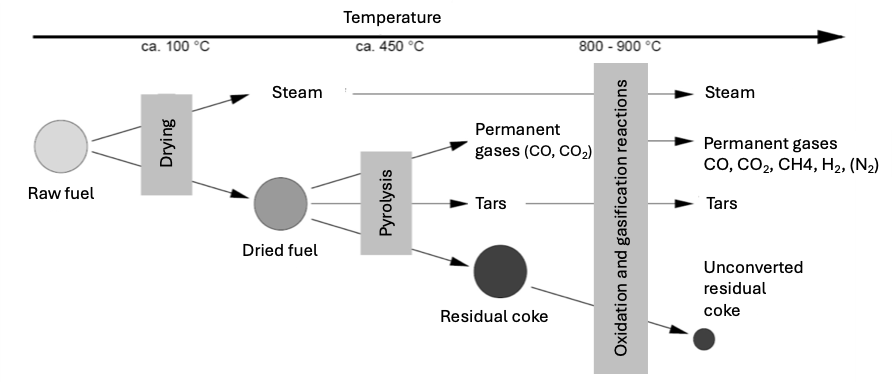
\includegraphics[width=\linewidth]{media/image1.png}

		\caption{Model course of heating, drying, and pyrolysis of the solid fuel and subsequent oxidation and gasification reactions (Tepper, 2005, p. 62).}

		\label{fig:rId7}


	\end{figure*}



	



	In the standard understanding of biomass gasification, we consider a clear sequence of events (Figure 1). First, water evaporates in the drying phase, followed by the pyrolysis phase where smaller organic compounds and gases like CO\textsubscript{2} and CO are released. Finally, in the redox phase, different gas particles react with each other and the particle surface. In the technical reactor, air is blown in from the bottom to the top and the wood pellets are filled in from above. Here, the sequence from drying to oxidation (Figure 1) follows the flow of the wood pellets through the reactor. In other words, oxidation occurs at the airflow side of the biomass bulk, and the reduction reactions that were of interest for my thesis predominantly happen in the large part of the biomass where the oxygen is exhausted. In this part of the reactor, the temperature is high enough to shift the reaction equilibrium to the side of burnable gases. With lower temperatures at the feed side, the main reactions are pyrolysis and drying, while a gas stream with tars, steam, and permanent gases leaves the reactor.



	While this model of the gasification suggests complex but distinct chemical reactions, I also clearly remember the time and smoky smell from cleaning the fume hood when the washer, a modified water canister, was overloaded by the gas flow and spit out a mix of tar and water to the ceiling. It became quite clear to me that engineering research looks quite different on paper than in reality. A mass balance that did not exactly add up and sealing rings that were not designed for such high temperatures were additional sources of frustration. Still, my findings were considered relevant for the large-scale reactor and the overall positive and sometimes humorous atmosphere of "The sheep fell sick again?" did a good job of brightening up the mood.



	\section{The popcorn effect}



	One particularly time-consuming aspect of my preparation was drying the wood pellets overnight. However, due to the additional time demands of cleaning and time lost to backlashes, I felt time pressure to complete my experiments within the scheduled 6 months of my thesis. To expedite the process, there were times I skipped the drying step, assuming the little moisture would evaporate before the pyrolysis and redox phases. Initially, this seemed inconsequential. However, upon closer analysis of my data and particles, I noticed an irregularity between my experiments, suggesting that the water content influenced the reactions and resulting gas mix. At further investigation, some wood particles from non-drying experiments appeared puffed up and the proportion of small particles increased by 16\% (Roßmann, 2012, p. 44). This hints at tar condensing in the drying phase at the particle surface, leading to a "popcorn effect".



	In the standard model, drying, pyrolysis, and redox reactions take place in sequential order, or respectively, at different areas within the bulk. In practice, however, I found that these processes are superimposed. Within the bulk, gaseous tar might condense and coat the particle surface during the drying phase. When hot water and tar then evaporate from the inner parts of these particles, they blow up like popcorn or break. Both cases increase the particle surface area in which the reactions of interest take place. In the oxygen-rich atmosphere, oxidation sets free more heat, further accelerating the oxidation and pyrolysis reactions. In the large part of the bulk, where oxygen is used up, the larger surface of puffed-up particles promotes reduction reactions, increasing the share of valuable burnable gases meant to fuel a combined heat and power unit. The discovery of superimposed water evaporation introduced the moist content of biomass as a relevant factor for the design and optimization of thermal biomass gasification.



	\begin{figure}
		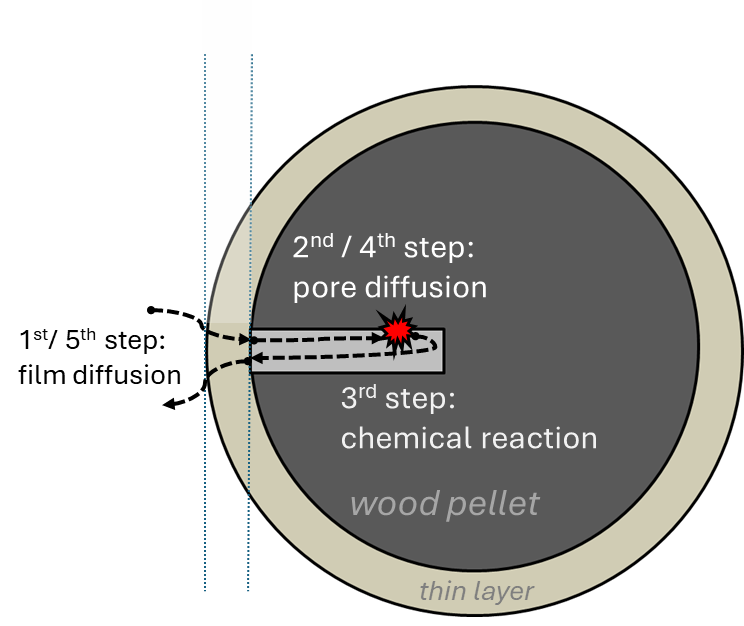
\includegraphics[width=\linewidth]{media/image2.png}

		\caption{Macro-kinetical reaction steps in the "shrinking core" model of gas-particle reactions (Roßmann, 2012, p. 22).}

		\label{fig:rId8}


	\end{figure}


	This finding of my bachelor thesis inspired subsequent research in that laboratory and confirmed initial speculations (Burhenne et al., 2013). While the macro-kinetical “shrinking core” model for gas-particle reactions describes diffusion processes and chemical reactions inside particles as limiting factors for the reaction speed (Figure 2), the case that an explosive expansion of water within the particle can “puff up” such channels, increase the inner surface, and affect the efficiency and type of gas produced, had not been discussed before. This discovery held potential implications for optimizing thermic gasification plants and other applications involving gas-particle reactions, such as catalysis or gas cleaning, ultimately aiding to reach technical and economic maturity.



	\section{Philosophical reflections on models, narratives, and scientific imagination}



	In the midst of what initially seemed like a devastating systemic error for my experiments and data, critical examination and a spark of inspiration led to subsequent research. It became evident that the model under discussion is -- like all models -- merely a simplified representation.



	In the realm of chemical engineering, a whole set of models is employed to represent and conceptualize the inner workings of a chemical reactor, encompassing gas flow models, heat and mass transfer to and within particles, as well as chemical micro- and macrokinetics, along with models focused on the thermic behavior of the reactor materials. Notably, reactor shape and alterations of airflow due to changes of particle size are not factored into models of chemical and kinetic equilibrium. Additionally, no computer simulation combines “all” models into a second reality. Instead, engineers employ a diverse set of models to focus on, discuss, and manipulate only those factors that seem relevant in the design, maintenance, or assessment process.



	Within the framework of my PhD thesis in philosophy, I argued that researchers and other stakeholders tell and share a set of stories to frame and give relevance to certain aspects of their models when developing or assessing emerging technologies (Roßmann, 2021). Narratives and models jointly guide and facilitate discussions of what should be imagined and believed at specific sites and circumstances, such as the drying, pyrolysis, or redox phases in the gasification of a woodchip. Consequently, established models and popular narratives of process steps, as well as earlier successes, accidents, and failures, establish norms for what is to be considered, expected, and imagined in the design process. In other words, narratives and models also constitute the canvas of ignorance that allows for the surprise of a serendipitous discovery (see Ross' comment on this anecdote; Ross, 2024). In the same vein, Stahl and Baier (2015) ask how many trial-and-error molecules it takes to tell a story that guides the choice of promising candidates in medical drug development.



	While the official models for thermic biomass gasification treat the phases as separate entities, the data obtained from varying the moisture content of the wood pellets prompted a reevaluation of the model's suitability for thermal biomass gasification in practice. Imagining the wood pellets to “puff up” like popcorn when the remaining water from an incomplete drying phase quickly evaporates was a compelling enough story to reconsider the model constraints of thermal gasification steps (Figure 1) and grasp the complex behavior of superimposed and mutually influencing processes. The analogy to puffing popcorn or the sensual imagery of cracking wood at a bonfire -- both outside the realm of a chemical engineering laboratory -- might have ignited the idea that such an effect is possible and, as means of communication, made the discussion with colleagues more relatable and engaging (Ross, 2024). The \emph{make-believe} that quickly evaporating water in such pores also “puffs up” wood pellets and increases their surface area, suggesting faster reactions, then fleshed out how this \emph{unconstrained analogy }(see Salis \& Frigg, 2020) can explain the relationship between accidental parameter variation and measurement data sufficiently to plan follow-up experiments.



	Challenging authorized models by drawing parallels between the behavior of wood pellets and popcorn, a concept seldom found in scientific theories, should not be dismissed as obvious. It was a bold claim of an undergrad student stretching conventions of discussing a chemical reactor. Also, philosophers often argue that imagination is only of epistemic value when it is constrained by certain rules: “It is generally agreed that imagination must be in some way constrained in order to be epistemically useful” (Badura \& Kind, 2021, p. 2). However, violating some rules does not disregard the value of such models or disregard all imaginative constraints, leading to free-floating fantastic imagination where wizards or fairies are held responsible for phenomena, such as puffing woodchips (Stuart, 2022). It rather aligns with Paul K. Feyerabend's notion to “respect your predecessors -- but don't be their slave!” (Feyerabend, 1985, p. 17). Introducing popcorn into the realm of redox reactions, shrinking particles, and Langmuir-Hinshelwood's mechanism was instrumental in producing testable ideas and certainly motivated by the collegial and sometimes humorous research environment, allowing for some creative variance in an otherwise more sterile technical imagination.



	\section{Conclusion}



	The popcorn effect in wood pellet gasification highlights the importance of creative analogies, imagination, and curiosity in scientific research. This serendipitous finding, born from a minor deviation in protocol, exemplifies the potential for unexpected observations to challenge established norms and advance our understanding of complex technical processes. Even though the thermal gasification of biomass did not reach commercial maturity in the 12 years since my bachelor thesis, research in the area continues in expectation of an energy crisis or more significant economic incentives for phosphorus recovery which may cause this niche technology to regain relevance.



	The conventional reporting of scientific discoveries often overlooks the speculative nature of hypotheses and narratives that shape the development of models. These elements can serve as foundations for unconventional ideas. My short discovery story highlights the need to allow space for humor and unconstrained imagination in scientific inquiry —an aspect that is often overlooked in documentation. By embracing this approach to share and reflect on the context of discovery, we not only enrich the research process but also create opportunities for little breakthroughs that might otherwise remain unnoticed.



	\section{Acknowledgments}



	I thank Stefan Gaillard for inviting me to not only tell but write down and further reflect on this anecdote. I thank Dr. Wendy Ross for her very rich and inspiring comment on this anecdote, which helped me to revise my philosophical reflection. Finally, I thank the H2020 ERC Synergy Grant No. 951393 for funding my research.



	\section{Bibliography}



	Badura, C., \& Kind, A. (Eds.). (2021). \emph{Epistemic uses of imagination}. Routledge.



	Burhenne, L., Damiani, M., \& Aicher, T. (2013). Effect of feedstock water content and pyrolysis temperature on the structure and reactivity of spruce wood char produced in fixed bed pyrolysis. \emph{Fuel}, \emph{107}, 836--847. \url{https://doi.org/10.1016/j.fuel.2013.01.033}



	Feyerabend, P. K. (1985).\emph{ Problems of Empiricism: Volume 2: Philosophical Papers}. Cambridge University Press.



	Lintner, C., Roßmann, M., \& Aicher, T. (2012). \emph{Integrale Klärschlammverwertung: Alternative Verwertungspfade für die Kläranlagen Breisach, Forchheim, Grezhausen und Grißheim}. Fraunhofer Institut für Solare Energiesysteme (ISE).



	Roser, M. (2020). Why did renewables become so cheap so fast? \emph{Our World in Data}. \url{https://ourworldindata.org/cheap-renewables-growth}



	Roßmann, M. (2012). \emph{Reduktionsreaktionen bei der Festbettvergasung von Biomasse} [Bachelor thesis]. Hochschule Mannheim.



	Roßmann, M. (2021). Vision as make-believe: How narratives and models represent sociotechnical futures. \emph{Journal of Responsible Innovation}, \emph{8}(1), 70--93. \url{https://doi.org/10.1080/23299460.2020.1853395}



	Salis, F., \& Frigg, R. (2020). Capturing the scientific imagination. In A. Levy \& P. Godfrey-Smith (Eds.), \emph{The Scientific Imagination} (pp. 17--50). Oxford University Press. \url{https://doi.org/10.1093/oso/9780190212308.003.0002}



	Stahl, M., \& Baier, S. (2015). How many molecules does it take to tell a story? Case studies, language, and an epistemic view of medicinal chemistry. \emph{ChemMedChem}, \emph{10}(6), 949--956. \url{https://doi.org/10.1002/cmdc.201500091}



	Stuart, M. T. (2022). Scientists are epistemic consequentialists about imagination. \emph{Philosophy of Science}, \emph{90}(3), 518-538. \url{https://doi.org/10.1017/psa.2022.31}



	Tan, Z., \& Lagerkvist, A. (2011). Phosphorus recovery from the biomass ash: A review. \emph{Renewable and Sustainable Energy Reviews}, \emph{15}(8), 3588--3602. \url{https://doi.org/10.1016/j.rser.2011.05.016}



	Tepper, H. (2005). \emph{Zur Vergasung von Rest- und Abfallholz in Wirbelschichtreaktoren für dezentrale Energieversorgungsanlagen }[Doctoral dissertation, Otto von Guericke University]. Universitätsbibliothek Otto von Guericke University Library. \url{https://doi.org/10.25673/4650}










\end{document}